% Options for packages loaded elsewhere
\PassOptionsToPackage{unicode}{hyperref}
\PassOptionsToPackage{hyphens}{url}
%
\documentclass[
]{article}
\usepackage{lmodern}
\usepackage{amssymb,amsmath}
\usepackage{ifxetex,ifluatex}
\ifnum 0\ifxetex 1\fi\ifluatex 1\fi=0 % if pdftex
  \usepackage[T1]{fontenc}
  \usepackage[utf8]{inputenc}
  \usepackage{textcomp} % provide euro and other symbols
\else % if luatex or xetex
  \usepackage{unicode-math}
  \defaultfontfeatures{Scale=MatchLowercase}
  \defaultfontfeatures[\rmfamily]{Ligatures=TeX,Scale=1}
\fi
% Use upquote if available, for straight quotes in verbatim environments
\IfFileExists{upquote.sty}{\usepackage{upquote}}{}
\IfFileExists{microtype.sty}{% use microtype if available
  \usepackage[]{microtype}
  \UseMicrotypeSet[protrusion]{basicmath} % disable protrusion for tt fonts
}{}
\makeatletter
\@ifundefined{KOMAClassName}{% if non-KOMA class
  \IfFileExists{parskip.sty}{%
    \usepackage{parskip}
  }{% else
    \setlength{\parindent}{0pt}
    \setlength{\parskip}{6pt plus 2pt minus 1pt}}
}{% if KOMA class
  \KOMAoptions{parskip=half}}
\makeatother
\usepackage{xcolor}
\IfFileExists{xurl.sty}{\usepackage{xurl}}{} % add URL line breaks if available
\IfFileExists{bookmark.sty}{\usepackage{bookmark}}{\usepackage{hyperref}}
\hypersetup{
  pdftitle={Solucionario: Segundo Parcial (30pts)},
  pdfauthor={Lic. Alvaro Chirino Gutierrez},
  hidelinks,
  pdfcreator={LaTeX via pandoc}}
\urlstyle{same} % disable monospaced font for URLs
\usepackage[margin=1in]{geometry}
\usepackage{color}
\usepackage{fancyvrb}
\newcommand{\VerbBar}{|}
\newcommand{\VERB}{\Verb[commandchars=\\\{\}]}
\DefineVerbatimEnvironment{Highlighting}{Verbatim}{commandchars=\\\{\}}
% Add ',fontsize=\small' for more characters per line
\usepackage{framed}
\definecolor{shadecolor}{RGB}{248,248,248}
\newenvironment{Shaded}{\begin{snugshade}}{\end{snugshade}}
\newcommand{\AlertTok}[1]{\textcolor[rgb]{0.94,0.16,0.16}{#1}}
\newcommand{\AnnotationTok}[1]{\textcolor[rgb]{0.56,0.35,0.01}{\textbf{\textit{#1}}}}
\newcommand{\AttributeTok}[1]{\textcolor[rgb]{0.77,0.63,0.00}{#1}}
\newcommand{\BaseNTok}[1]{\textcolor[rgb]{0.00,0.00,0.81}{#1}}
\newcommand{\BuiltInTok}[1]{#1}
\newcommand{\CharTok}[1]{\textcolor[rgb]{0.31,0.60,0.02}{#1}}
\newcommand{\CommentTok}[1]{\textcolor[rgb]{0.56,0.35,0.01}{\textit{#1}}}
\newcommand{\CommentVarTok}[1]{\textcolor[rgb]{0.56,0.35,0.01}{\textbf{\textit{#1}}}}
\newcommand{\ConstantTok}[1]{\textcolor[rgb]{0.00,0.00,0.00}{#1}}
\newcommand{\ControlFlowTok}[1]{\textcolor[rgb]{0.13,0.29,0.53}{\textbf{#1}}}
\newcommand{\DataTypeTok}[1]{\textcolor[rgb]{0.13,0.29,0.53}{#1}}
\newcommand{\DecValTok}[1]{\textcolor[rgb]{0.00,0.00,0.81}{#1}}
\newcommand{\DocumentationTok}[1]{\textcolor[rgb]{0.56,0.35,0.01}{\textbf{\textit{#1}}}}
\newcommand{\ErrorTok}[1]{\textcolor[rgb]{0.64,0.00,0.00}{\textbf{#1}}}
\newcommand{\ExtensionTok}[1]{#1}
\newcommand{\FloatTok}[1]{\textcolor[rgb]{0.00,0.00,0.81}{#1}}
\newcommand{\FunctionTok}[1]{\textcolor[rgb]{0.00,0.00,0.00}{#1}}
\newcommand{\ImportTok}[1]{#1}
\newcommand{\InformationTok}[1]{\textcolor[rgb]{0.56,0.35,0.01}{\textbf{\textit{#1}}}}
\newcommand{\KeywordTok}[1]{\textcolor[rgb]{0.13,0.29,0.53}{\textbf{#1}}}
\newcommand{\NormalTok}[1]{#1}
\newcommand{\OperatorTok}[1]{\textcolor[rgb]{0.81,0.36,0.00}{\textbf{#1}}}
\newcommand{\OtherTok}[1]{\textcolor[rgb]{0.56,0.35,0.01}{#1}}
\newcommand{\PreprocessorTok}[1]{\textcolor[rgb]{0.56,0.35,0.01}{\textit{#1}}}
\newcommand{\RegionMarkerTok}[1]{#1}
\newcommand{\SpecialCharTok}[1]{\textcolor[rgb]{0.00,0.00,0.00}{#1}}
\newcommand{\SpecialStringTok}[1]{\textcolor[rgb]{0.31,0.60,0.02}{#1}}
\newcommand{\StringTok}[1]{\textcolor[rgb]{0.31,0.60,0.02}{#1}}
\newcommand{\VariableTok}[1]{\textcolor[rgb]{0.00,0.00,0.00}{#1}}
\newcommand{\VerbatimStringTok}[1]{\textcolor[rgb]{0.31,0.60,0.02}{#1}}
\newcommand{\WarningTok}[1]{\textcolor[rgb]{0.56,0.35,0.01}{\textbf{\textit{#1}}}}
\usepackage{graphicx,grffile}
\makeatletter
\def\maxwidth{\ifdim\Gin@nat@width>\linewidth\linewidth\else\Gin@nat@width\fi}
\def\maxheight{\ifdim\Gin@nat@height>\textheight\textheight\else\Gin@nat@height\fi}
\makeatother
% Scale images if necessary, so that they will not overflow the page
% margins by default, and it is still possible to overwrite the defaults
% using explicit options in \includegraphics[width, height, ...]{}
\setkeys{Gin}{width=\maxwidth,height=\maxheight,keepaspectratio}
% Set default figure placement to htbp
\makeatletter
\def\fps@figure{htbp}
\makeatother
\setlength{\emergencystretch}{3em} % prevent overfull lines
\providecommand{\tightlist}{%
  \setlength{\itemsep}{0pt}\setlength{\parskip}{0pt}}
\setcounter{secnumdepth}{-\maxdimen} % remove section numbering

\title{Solucionario: Segundo Parcial (30pts)}
\usepackage{etoolbox}
\makeatletter
\providecommand{\subtitle}[1]{% add subtitle to \maketitle
  \apptocmd{\@title}{\par {\large #1 \par}}{}{}
}
\makeatother
\subtitle{Programacion Estadística I}
\author{Lic. Alvaro Chirino Gutierrez}
\date{17/7/2020}

\begin{document}
\maketitle

\hypertarget{pregunta-1-5-pts}{%
\section{Pregunta 1 (5 pts)}\label{pregunta-1-5-pts}}

\begin{itemize}
\tightlist
\item
  (1pts) Describa la diferencia entre los procesos de inferencia:
  descriptiva, causal y predictivo
\item
  (1pts) De un ejemplo de record linkage
\item
  (2pts) Describa los errores de fila, columna y celda
\item
  (1pts) Describa los errores asociados a las 3 V en big data
\end{itemize}

\hypertarget{pregunta-2-10-pts}{%
\section{Pregunta 2 (10 pts)}\label{pregunta-2-10-pts}}

\begin{itemize}
\tightlist
\item
  (5pts) Usando la base de datos de computo para las elecciones del 20
  de octubre de 2019:
\end{itemize}

Solución,

\begin{Shaded}
\begin{Highlighting}[]
\KeywordTok{rm}\NormalTok{(}\DataTypeTok{list=}\KeywordTok{ls}\NormalTok{())}
\CommentTok{# 1. Cargue la base en R}
\KeywordTok{load}\NormalTok{(}\StringTok{"C:}\CharTok{\textbackslash{}\textbackslash{}}\StringTok{Users}\CharTok{\textbackslash{}\textbackslash{}}\StringTok{ALVARO}\CharTok{\textbackslash{}\textbackslash{}}\StringTok{Documents}\CharTok{\textbackslash{}\textbackslash{}}\StringTok{GitHub}\CharTok{\textbackslash{}\textbackslash{}}\StringTok{EST-383}\CharTok{\textbackslash{}\textbackslash{}}\StringTok{data}\CharTok{\textbackslash{}\textbackslash{}}\StringTok{oct20.RData"}\NormalTok{)}
\CommentTok{#2. Guarde la base en csv}
\KeywordTok{setwd}\NormalTok{(}\StringTok{"C:}\CharTok{\textbackslash{}\textbackslash{}}\StringTok{Users}\CharTok{\textbackslash{}\textbackslash{}}\StringTok{ALVARO}\CharTok{\textbackslash{}\textbackslash{}}\StringTok{Documents}\CharTok{\textbackslash{}\textbackslash{}}\StringTok{GitHub}\CharTok{\textbackslash{}\textbackslash{}}\StringTok{EST-383}\CharTok{\textbackslash{}\textbackslash{}}\StringTok{parciales"}\NormalTok{)}
\KeywordTok{write.csv}\NormalTok{(computo,}\StringTok{"computo.csv"}\NormalTok{)}
\CommentTok{#3. Cargue el csv como un objeto ffdf. Con el nombre bd1.}
\KeywordTok{library}\NormalTok{(ffbase)}
\end{Highlighting}
\end{Shaded}

\begin{verbatim}
## Loading required package: ff
\end{verbatim}

\begin{verbatim}
## Loading required package: bit
\end{verbatim}

\begin{verbatim}
## Attaching package bit
\end{verbatim}

\begin{verbatim}
## package:bit (c) 2008-2012 Jens Oehlschlaegel (GPL-2)
\end{verbatim}

\begin{verbatim}
## creators: bit bitwhich
\end{verbatim}

\begin{verbatim}
## coercion: as.logical as.integer as.bit as.bitwhich which
\end{verbatim}

\begin{verbatim}
## operator: ! & | xor != ==
\end{verbatim}

\begin{verbatim}
## querying: print length any all min max range sum summary
\end{verbatim}

\begin{verbatim}
## bit access: length<- [ [<- [[ [[<-
\end{verbatim}

\begin{verbatim}
## for more help type ?bit
\end{verbatim}

\begin{verbatim}
## 
## Attaching package: 'bit'
\end{verbatim}

\begin{verbatim}
## The following object is masked from 'package:base':
## 
##     xor
\end{verbatim}

\begin{verbatim}
## Attaching package ff
\end{verbatim}

\begin{verbatim}
## - getOption("fftempdir")=="C:/Users/ALVARO/AppData/Local/Temp/Rtmp0qHr9r"
\end{verbatim}

\begin{verbatim}
## - getOption("ffextension")=="ff"
\end{verbatim}

\begin{verbatim}
## - getOption("ffdrop")==TRUE
\end{verbatim}

\begin{verbatim}
## - getOption("fffinonexit")==TRUE
\end{verbatim}

\begin{verbatim}
## - getOption("ffpagesize")==65536
\end{verbatim}

\begin{verbatim}
## - getOption("ffcaching")=="mmnoflush"  -- consider "ffeachflush" if your system stalls on large writes
\end{verbatim}

\begin{verbatim}
## - getOption("ffbatchbytes")==84641054.72 -- consider a different value for tuning your system
\end{verbatim}

\begin{verbatim}
## - getOption("ffmaxbytes")==4232052736 -- consider a different value for tuning your system
\end{verbatim}

\begin{verbatim}
## 
## Attaching package: 'ff'
\end{verbatim}

\begin{verbatim}
## The following objects are masked from 'package:bit':
## 
##     clone, clone.default, clone.list
\end{verbatim}

\begin{verbatim}
## The following objects are masked from 'package:utils':
## 
##     write.csv, write.csv2
\end{verbatim}

\begin{verbatim}
## The following objects are masked from 'package:base':
## 
##     is.factor, is.ordered
\end{verbatim}

\begin{verbatim}
## Registered S3 methods overwritten by 'ffbase':
##   method   from
##   [.ff     ff  
##   [.ffdf   ff  
##   [<-.ff   ff  
##   [<-.ffdf ff
\end{verbatim}

\begin{verbatim}
## 
## Attaching package: 'ffbase'
\end{verbatim}

\begin{verbatim}
## The following objects are masked from 'package:ff':
## 
##     [.ff, [.ffdf, [<-.ff, [<-.ffdf
\end{verbatim}

\begin{verbatim}
## The following objects are masked from 'package:base':
## 
##     %in%, table
\end{verbatim}

\begin{Shaded}
\begin{Highlighting}[]
\KeywordTok{library}\NormalTok{(ff)}
\KeywordTok{system}\NormalTok{(}\StringTok{"mkdir ffdf"}\NormalTok{)}
\end{Highlighting}
\end{Shaded}

\begin{verbatim}
## [1] 1
\end{verbatim}

\begin{Shaded}
\begin{Highlighting}[]
\KeywordTok{options}\NormalTok{(}\DataTypeTok{fftempdir=}\StringTok{"C:}\CharTok{\textbackslash{}\textbackslash{}}\StringTok{Users}\CharTok{\textbackslash{}\textbackslash{}}\StringTok{ALVARO}\CharTok{\textbackslash{}\textbackslash{}}\StringTok{Documents}\CharTok{\textbackslash{}\textbackslash{}}\StringTok{GitHub}\CharTok{\textbackslash{}\textbackslash{}}\StringTok{EST-383}\CharTok{\textbackslash{}\textbackslash{}}\StringTok{parciales}\CharTok{\textbackslash{}\textbackslash{}}\StringTok{ffdf"}\NormalTok{)}
\NormalTok{bd1<-}\KeywordTok{read.csv.ffdf}\NormalTok{(}\DataTypeTok{file=}\StringTok{"computo.csv"}\NormalTok{,}\DataTypeTok{sep=}\StringTok{","}\NormalTok{,}\DataTypeTok{header=}\NormalTok{T,}\DataTypeTok{colClasses=}\OtherTok{NA}\NormalTok{)}
\CommentTok{# 4. Sobre el objeto bd1 obtenga una tabla de departamento vs. tipo de elección}
\KeywordTok{head}\NormalTok{(}\KeywordTok{table}\NormalTok{(bd1}\OperatorTok{$}\NormalTok{Departamento,bd1}\OperatorTok{$}\NormalTok{Elección))}
\end{Highlighting}
\end{Shaded}

\begin{verbatim}
##               
##                Diputados Uninominales Presidente y Vicepresidente
##   Berlín                            0                           2
##   Bruselas                          0                           1
##   Buenos Aires                      0                         532
##   Chubut                            0                          14
##   Chuquisaca                     1828                        1828
##   Cordoba                           0                          22
##               
##                Diputados Especiales
##   Berlín                          0
##   Bruselas                        0
##   Buenos Aires                    0
##   Chubut                          0
##   Chuquisaca                      0
##   Cordoba                         0
\end{verbatim}

\begin{Shaded}
\begin{Highlighting}[]
\CommentTok{# 5. Repita el paso 4 con una base obtenida con el comando as.ffdf o as.data.frame.ffdf}
\NormalTok{bd2<-}\KeywordTok{as.data.frame}\NormalTok{(bd1)}
\NormalTok{bd2<-}\KeywordTok{as.ffdf}\NormalTok{(bd2)}
\KeywordTok{head}\NormalTok{(}\KeywordTok{table}\NormalTok{(bd2}\OperatorTok{$}\NormalTok{Departamento,bd2}\OperatorTok{$}\NormalTok{Elección))}
\end{Highlighting}
\end{Shaded}

\begin{verbatim}
##               
##                Diputados Uninominales Presidente y Vicepresidente
##   Berlín                            0                           2
##   Bruselas                          0                           1
##   Buenos Aires                      0                         532
##   Chubut                            0                          14
##   Chuquisaca                     1828                        1828
##   Cordoba                           0                          22
##               
##                Diputados Especiales
##   Berlín                          0
##   Bruselas                        0
##   Buenos Aires                    0
##   Chubut                          0
##   Chuquisaca                      0
##   Cordoba                         0
\end{verbatim}

\begin{Shaded}
\begin{Highlighting}[]
\CommentTok{#otra alternativa}
\NormalTok{aux<-}\KeywordTok{sapply}\NormalTok{(computo,is.character)}\CommentTok{#character a factor}
\ControlFlowTok{for}\NormalTok{(i }\ControlFlowTok{in} \KeywordTok{names}\NormalTok{(computo))\{}
  \ControlFlowTok{if}\NormalTok{(aux[i]}\OperatorTok{==}\NormalTok{T)\{}
\NormalTok{    computo[,i]<-}\KeywordTok{as.factor}\NormalTok{(computo[,i])}
\NormalTok{  \}}
\NormalTok{\}}
\NormalTok{bd3<-}\KeywordTok{as.ffdf}\NormalTok{(computo)}
\KeywordTok{head}\NormalTok{(}\KeywordTok{table}\NormalTok{(bd3}\OperatorTok{$}\NormalTok{Departamento,bd3}\OperatorTok{$}\NormalTok{Elección))}
\end{Highlighting}
\end{Shaded}

\begin{verbatim}
##              
##               Diputados Especiales Diputados Uninominales
##   Acre                           0                      0
##   Andalucia                      0                      0
##   Antofagasta                    0                      0
##   Arica                          0                      0
##   Atacama                        0                      0
##   Beijing                        0                      0
##              
##               Presidente y Vicepresidente
##   Acre                                  1
##   Andalucia                            22
##   Antofagasta                          68
##   Arica                                14
##   Atacama                               6
##   Beijing                               1
\end{verbatim}

\begin{itemize}
\tightlist
\item
  (5pts) Usando la base de datos de computo para las elecciones del 20
  de octubre de 2019. Seleccione solo Bolivia y las elecciones de
  presidente y vicepresidente.
\end{itemize}

Solución,

\begin{verbatim}
## $Duration
##    user  system elapsed 
##    0.02    0.00    0.02 
## 
## $Result
##     Inscritos            CC           FPV           MTS           UCS 
##       6973768       2186326         23028         75529         24007 
##    MAS - IPSP           21F           PDC           MNR       PAN-BOL 
##       2768427        256833        522576         41033         37841 
## Votos Válidos       Blancos         Nulos 
##       5935944         91610        222856
\end{verbatim}

\begin{verbatim}
## $Duration
##    user  system elapsed 
##    0.03    0.00    0.03 
## 
## $Result
##            CC           FPV           MTS           UCS    MAS - IPSP 
##    66.1640843     0.6968890     2.2857100     0.7265162    83.7800206 
##           21F           PDC           MNR       PAN-BOL Votos Válidos 
##     7.7724549    15.8145503     1.2417686     1.1451701   179.6375741 
##       Blancos         Nulos 
##     2.7723641     6.7442198
\end{verbatim}

\hypertarget{pregunta-3-15-pts}{%
\section{Pregunta 3 (15 pts)}\label{pregunta-3-15-pts}}

\begin{itemize}
\tightlist
\item
  (5 pts) Usando la encuesta de hogares defina una base de datos que
  contenga las siguientes variables para los jefes de hogar:

  \begin{itemize}
  \tightlist
  \item
    Edad
  \item
    Sexo
  \item
    Ingreso laboral
  \item
    Departamento
  \item
    Años de educación
  \item
    Área
  \item
    Incidencia de pobreza moderada (p0)
  \item
    Acceso a internet en el hogar
  \item
    Vivienda propia y totalmente pagada
  \item
    Número de miembros en el hogar
  \end{itemize}
\end{itemize}

(Sugerencia: Use la variable folio y el comando merge para unir bases)

Solución,

\begin{Shaded}
\begin{Highlighting}[]
\KeywordTok{rm}\NormalTok{(}\DataTypeTok{list=}\KeywordTok{ls}\NormalTok{())}
\KeywordTok{load}\NormalTok{(}\KeywordTok{url}\NormalTok{(}\StringTok{"https://github.com/AlvaroLimber/EST-383/raw/master/data/eh18.Rdata"}\NormalTok{))}
\CommentTok{#jefe/a del hogar}
\NormalTok{jefe<-eh18p }\OperatorTok\StringTok{ }\KeywordTok{filter}\NormalTok{(s02a_}\DecValTok{05}\OperatorTok{==}\KeywordTok{unique}\NormalTok{(eh18p}\OperatorTok{$}\NormalTok{s02a_}\DecValTok{05}\NormalTok{)[}\DecValTok{1}\NormalTok{]) }\OperatorTok\StringTok{ }\KeywordTok{select}\NormalTok{(folio,s02a_}\DecValTok{02}\NormalTok{,s02a_}\DecValTok{03}\NormalTok{,ylab,depto,aestudio,area,p0)}
\CommentTok{#variables en la vivienda}
\NormalTok{vv<-eh18v }\OperatorTok\StringTok{ }\KeywordTok{mutate}\NormalTok{(}\DataTypeTok{internet=}\NormalTok{s01a_}\DecValTok{31}\OperatorTok{==}\StringTok{"1. Si"}\NormalTok{, }\DataTypeTok{vpropia=}\NormalTok{(s01a_}\DecValTok{02}\OperatorTok{==}\StringTok{ }\KeywordTok{unique}\NormalTok{(eh18v}\OperatorTok{$}\NormalTok{s01a_}\DecValTok{02}\NormalTok{)[}\DecValTok{1}\NormalTok{])) }\OperatorTok\StringTok{ }\KeywordTok{select}\NormalTok{(folio,internet,vpropia)}
\CommentTok{#miembros}
\NormalTok{mm<-eh18p }\OperatorTok\StringTok{ }\KeywordTok{mutate}\NormalTok{(}\DataTypeTok{miembros=}\DecValTok{1}\NormalTok{) }\OperatorTok\StringTok{ }\KeywordTok{group_by}\NormalTok{(folio) }\OperatorTok\StringTok{ }\KeywordTok{summarise}\NormalTok{(}\DataTypeTok{miembros=}\KeywordTok{sum}\NormalTok{(miembros))}
\end{Highlighting}
\end{Shaded}

\begin{verbatim}
## `summarise()` ungrouping output (override with `.groups` argument)
\end{verbatim}

\begin{Shaded}
\begin{Highlighting}[]
\CommentTok{#base consolidada}
\NormalTok{jefe<-}\KeywordTok{merge}\NormalTok{(jefe,mm)}
\NormalTok{jefe<-}\KeywordTok{merge}\NormalTok{(jefe,vv)}
\KeywordTok{head}\NormalTok{(jefe)}
\end{Highlighting}
\end{Shaded}

\begin{verbatim}
##                    folio  s02a_02 s02a_03    ylab      depto aestudio   area
## 1 111-00419704629-A-0011 1.Hombre      60 2256.00 Chuquisaca        2 Urbana
## 2 111-00419704629-A-0021 1.Hombre      36 2446.45 Chuquisaca        0 Urbana
## 3 111-00419704629-A-0041 1.Hombre      25 2598.00 Chuquisaca       12 Urbana
## 4 111-00419704629-A-0051 1.Hombre      47 2060.00 Chuquisaca        5 Urbana
## 5 111-00419704629-A-0071 1.Hombre      23 2060.00 Chuquisaca        8 Urbana
## 6 111-00419704629-A-0081 1.Hombre      49 2500.00 Chuquisaca        4 Urbana
##         p0 miembros internet vpropia
## 1 No Pobre        2    FALSE    TRUE
## 2    Pobre        5    FALSE   FALSE
## 3 No Pobre        4    FALSE   FALSE
## 4    Pobre        3    FALSE    TRUE
## 5    Pobre        4    FALSE   FALSE
## 6 No Pobre        4    FALSE    TRUE
\end{verbatim}

\begin{itemize}
\tightlist
\item
  (10 pts) Para la base alojada en R y la base alojada en Spark, genere
  lo siguiente:
\end{itemize}

\begin{Shaded}
\begin{Highlighting}[]
\KeywordTok{rm}\NormalTok{(eh18p,eh18v,mm,vv)}
\KeywordTok{library}\NormalTok{(sparklyr)}
\NormalTok{sc<-}\KeywordTok{spark_connect}\NormalTok{(}\DataTypeTok{master=}\StringTok{"local"}\NormalTok{)}
\NormalTok{sp_jefe<-}\KeywordTok{copy_to}\NormalTok{(sc,jefe,}\StringTok{"eh18"}\NormalTok{)}
\CommentTok{# Promedio de años de educación del jefe del hogar por departamento y Área }
\CommentTok{#R}
\NormalTok{jefe }\OperatorTok\StringTok{ }\KeywordTok{group_by}\NormalTok{(depto,area) }\OperatorTok\StringTok{ }\KeywordTok{summarise}\NormalTok{(}\KeywordTok{mean}\NormalTok{(aestudio,}\DataTypeTok{na.rm=}\NormalTok{T))}
\end{Highlighting}
\end{Shaded}

\begin{verbatim}
## `summarise()` regrouping output by 'depto' (override with `.groups` argument)
\end{verbatim}

\begin{verbatim}
## # A tibble: 18 x 3
## # Groups:   depto [9]
##    depto      area   `mean(aestudio, na.rm = T)`
##    <fct>      <fct>                        <dbl>
##  1 Chuquisaca Urbana                       10.5 
##  2 Chuquisaca Rural                         4.92
##  3 La Paz     Urbana                       10.8 
##  4 La Paz     Rural                         6.73
##  5 Cochabamba Urbana                       10.5 
##  6 Cochabamba Rural                         5.09
##  7 Oruro      Urbana                       10.9 
##  8 Oruro      Rural                         6.89
##  9 Potosí     Urbana                        9.36
## 10 Potosí     Rural                         5.29
## 11 Tarija     Urbana                       10.3 
## 12 Tarija     Rural                         5.74
## 13 Santa Cruz Urbana                       10.5 
## 14 Santa Cruz Rural                         6.76
## 15 Beni       Urbana                       10.5 
## 16 Beni       Rural                         7.93
## 17 Pando      Urbana                       11.7 
## 18 Pando      Rural                         8.09
\end{verbatim}

\begin{Shaded}
\begin{Highlighting}[]
\CommentTok{#Spark}
\NormalTok{sp_jefe }\OperatorTok\StringTok{ }\KeywordTok{group_by}\NormalTok{(depto,area) }\OperatorTok\StringTok{ }\KeywordTok{summarise}\NormalTok{(}\KeywordTok{mean}\NormalTok{(aestudio))}
\end{Highlighting}
\end{Shaded}

\begin{verbatim}
## Warning: Missing values are always removed in SQL.
## Use `mean(x, na.rm = TRUE)` to silence this warning
## This warning is displayed only once per session.
\end{verbatim}

\begin{verbatim}
## # Source: spark<?> [?? x 3]
## # Groups: depto
##    depto      area   `mean(aestudio)`
##    <chr>      <chr>             <dbl>
##  1 Chuquisaca Rural              4.92
##  2 La Paz     Rural              6.73
##  3 Oruro      Urbana            10.9 
##  4 Tarija     Urbana            10.3 
##  5 Santa Cruz Urbana            10.5 
##  6 Beni       Urbana            10.5 
##  7 Pando      Urbana            11.7 
##  8 Pando      Rural              8.09
##  9 La Paz     Urbana            10.8 
## 10 Potosí     Urbana             9.36
## # ... with more rows
\end{verbatim}

\begin{Shaded}
\begin{Highlighting}[]
\CommentTok{# Proporción de jefes del hogar con un ingreso laboral superior a 4000 Bs. Por Departamento y Sexo }
\CommentTok{#R}
\NormalTok{jefe }\OperatorTok\StringTok{ }\KeywordTok{mutate}\NormalTok{(}\DataTypeTok{pp=}\NormalTok{ylab}\OperatorTok{>}\DecValTok{4000}\NormalTok{) }\OperatorTok\StringTok{ }\KeywordTok{group_by}\NormalTok{(depto,s02a_}\DecValTok{02}\NormalTok{) }\OperatorTok\StringTok{ }\KeywordTok{summarise}\NormalTok{(}\KeywordTok{mean}\NormalTok{(pp,}\DataTypeTok{na.rm=}\NormalTok{T))}
\end{Highlighting}
\end{Shaded}

\begin{verbatim}
## `summarise()` regrouping output by 'depto' (override with `.groups` argument)
\end{verbatim}

\begin{verbatim}
## # A tibble: 18 x 3
## # Groups:   depto [9]
##    depto      s02a_02  `mean(pp, na.rm = T)`
##    <fct>      <fct>                    <dbl>
##  1 Chuquisaca 1.Hombre                 0.214
##  2 Chuquisaca 2.Mujer                  0.222
##  3 La Paz     1.Hombre                 0.272
##  4 La Paz     2.Mujer                  0.153
##  5 Cochabamba 1.Hombre                 0.276
##  6 Cochabamba 2.Mujer                  0.173
##  7 Oruro      1.Hombre                 0.249
##  8 Oruro      2.Mujer                  0.203
##  9 Potosí     1.Hombre                 0.226
## 10 Potosí     2.Mujer                  0.125
## 11 Tarija     1.Hombre                 0.321
## 12 Tarija     2.Mujer                  0.175
## 13 Santa Cruz 1.Hombre                 0.315
## 14 Santa Cruz 2.Mujer                  0.206
## 15 Beni       1.Hombre                 0.267
## 16 Beni       2.Mujer                  0.204
## 17 Pando      1.Hombre                 0.286
## 18 Pando      2.Mujer                  0.25
\end{verbatim}

\begin{Shaded}
\begin{Highlighting}[]
\CommentTok{#Spark}
\NormalTok{sp_jefe }\OperatorTok\StringTok{ }\KeywordTok{mutate}\NormalTok{(}\DataTypeTok{pp=}\KeywordTok{ifelse}\NormalTok{(ylab}\OperatorTok{>}\DecValTok{4000}\NormalTok{,}\DecValTok{1}\NormalTok{,}\DecValTok{0}\NormalTok{)) }\OperatorTok\StringTok{ }\KeywordTok{group_by}\NormalTok{(depto,s02a_}\DecValTok{02}\NormalTok{) }\OperatorTok\StringTok{ }\KeywordTok{summarise}\NormalTok{(}\KeywordTok{mean}\NormalTok{(pp))}
\end{Highlighting}
\end{Shaded}

\begin{verbatim}
## # Source: spark<?> [?? x 3]
## # Groups: depto
##    depto      s02a_02  `mean(pp)`
##    <chr>      <chr>         <dbl>
##  1 Chuquisaca 2.Mujer       0.222
##  2 Potosí     2.Mujer       0.125
##  3 Tarija     2.Mujer       0.175
##  4 La Paz     1.Hombre      0.272
##  5 Cochabamba 1.Hombre      0.276
##  6 Oruro      2.Mujer       0.203
##  7 Tarija     1.Hombre      0.321
##  8 Beni       2.Mujer       0.204
##  9 Chuquisaca 1.Hombre      0.214
## 10 Oruro      1.Hombre      0.249
## # ... with more rows
\end{verbatim}

\begin{Shaded}
\begin{Highlighting}[]
\CommentTok{# Proporción de pobreza moderada en hogares con jefes de hogar de 30 años o menos por sexo }
\NormalTok{jefe }\OperatorTok\StringTok{ }\KeywordTok{mutate}\NormalTok{(}\DataTypeTok{p0=}\KeywordTok{ifelse}\NormalTok{(p0}\OperatorTok{==}\StringTok{"Pobre"}\NormalTok{,}\DecValTok{1}\NormalTok{,}\DecValTok{0}\NormalTok{)) }\OperatorTok\StringTok{ }\KeywordTok{filter}\NormalTok{(s02a_}\DecValTok{03}\OperatorTok{<=}\DecValTok{30}\NormalTok{) }\OperatorTok\StringTok{ }\KeywordTok{group_by}\NormalTok{(s02a_}\DecValTok{02}\NormalTok{)}\OperatorTok\StringTok{ }\KeywordTok{summarise}\NormalTok{(}\KeywordTok{mean}\NormalTok{(p0))}
\end{Highlighting}
\end{Shaded}

\begin{verbatim}
## `summarise()` ungrouping output (override with `.groups` argument)
\end{verbatim}

\begin{verbatim}
## # A tibble: 2 x 2
##   s02a_02  `mean(p0)`
##   <fct>         <dbl>
## 1 1.Hombre      0.248
## 2 2.Mujer       0.312
\end{verbatim}

\begin{Shaded}
\begin{Highlighting}[]
\NormalTok{sp_jefe }\OperatorTok\StringTok{ }\KeywordTok{mutate}\NormalTok{(}\DataTypeTok{p0=}\KeywordTok{ifelse}\NormalTok{(p0}\OperatorTok{==}\StringTok{"Pobre"}\NormalTok{,}\DecValTok{1}\NormalTok{,}\DecValTok{0}\NormalTok{)) }\OperatorTok\StringTok{ }\KeywordTok{filter}\NormalTok{(s02a_}\DecValTok{03}\OperatorTok{<=}\DecValTok{30}\NormalTok{) }\OperatorTok\StringTok{ }\KeywordTok{group_by}\NormalTok{(s02a_}\DecValTok{02}\NormalTok{)}\OperatorTok\StringTok{ }\KeywordTok{summarise}\NormalTok{(}\KeywordTok{mean}\NormalTok{(p0))}
\end{Highlighting}
\end{Shaded}

\begin{verbatim}
## # Source: spark<?> [?? x 2]
##   s02a_02  `mean(p0)`
##   <chr>         <dbl>
## 1 2.Mujer       0.312
## 2 1.Hombre      0.248
\end{verbatim}

\begin{Shaded}
\begin{Highlighting}[]
\CommentTok{# Promedio de miembros en el hogar por departamento, área y sexo del jefe del hogar}
\NormalTok{jefe }\OperatorTok\StringTok{ }\KeywordTok{group_by}\NormalTok{(depto,area,s02a_}\DecValTok{02}\NormalTok{) }\OperatorTok\StringTok{ }\KeywordTok{summarise}\NormalTok{(}\KeywordTok{mean}\NormalTok{(miembros))}
\end{Highlighting}
\end{Shaded}

\begin{verbatim}
## `summarise()` regrouping output by 'depto', 'area' (override with `.groups` argument)
\end{verbatim}

\begin{verbatim}
## # A tibble: 36 x 4
## # Groups:   depto, area [18]
##    depto      area   s02a_02  `mean(miembros)`
##    <fct>      <fct>  <fct>               <dbl>
##  1 Chuquisaca Urbana 1.Hombre             3.58
##  2 Chuquisaca Urbana 2.Mujer              2.64
##  3 Chuquisaca Rural  1.Hombre             3.92
##  4 Chuquisaca Rural  2.Mujer              2.65
##  5 La Paz     Urbana 1.Hombre             3.67
##  6 La Paz     Urbana 2.Mujer              2.88
##  7 La Paz     Rural  1.Hombre             3.26
##  8 La Paz     Rural  2.Mujer              2.52
##  9 Cochabamba Urbana 1.Hombre             3.60
## 10 Cochabamba Urbana 2.Mujer              2.89
## # ... with 26 more rows
\end{verbatim}

\begin{Shaded}
\begin{Highlighting}[]
\NormalTok{sp_jefe }\OperatorTok\StringTok{ }\KeywordTok{group_by}\NormalTok{(depto,area,s02a_}\DecValTok{02}\NormalTok{) }\OperatorTok\StringTok{ }\KeywordTok{summarise}\NormalTok{(}\KeywordTok{mean}\NormalTok{(miembros))}
\end{Highlighting}
\end{Shaded}

\begin{verbatim}
## # Source: spark<?> [?? x 4]
## # Groups: depto, area
##    depto      area   s02a_02  `mean(miembros)`
##    <chr>      <chr>  <chr>               <dbl>
##  1 Chuquisaca Urbana 2.Mujer              2.64
##  2 La Paz     Urbana 1.Hombre             3.67
##  3 La Paz     Rural  1.Hombre             3.26
##  4 Cochabamba Urbana 2.Mujer              2.89
##  5 Cochabamba Urbana 1.Hombre             3.60
##  6 Potosí     Urbana 1.Hombre             3.85
##  7 Santa Cruz Rural  1.Hombre             3.39
##  8 Chuquisaca Rural  1.Hombre             3.92
##  9 La Paz     Urbana 2.Mujer              2.88
## 10 Cochabamba Rural  1.Hombre             3.41
## # ... with more rows
\end{verbatim}

\begin{Shaded}
\begin{Highlighting}[]
\CommentTok{# Gráfico sobre el acceso al internet por departamento (ggplot)}
\KeywordTok{library}\NormalTok{(ggplot2)}
\KeywordTok{ggplot}\NormalTok{(jefe,}\KeywordTok{aes}\NormalTok{(internet))}\OperatorTok{+}\KeywordTok{geom_bar}\NormalTok{()}\OperatorTok{+}\KeywordTok{facet_wrap}\NormalTok{(}\OperatorTok{~}\NormalTok{depto)}
\end{Highlighting}
\end{Shaded}

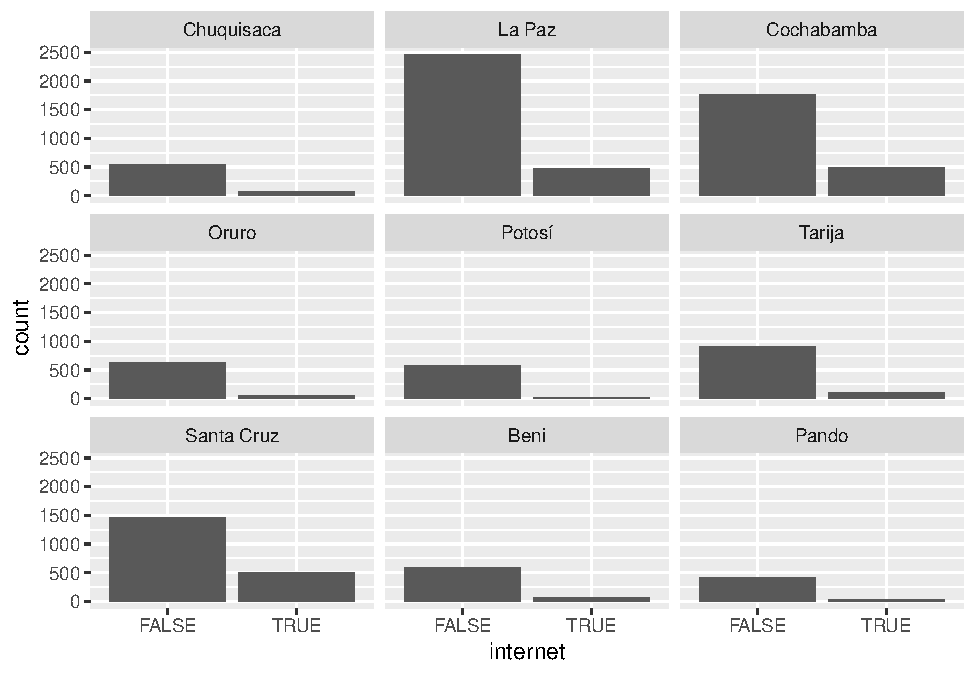
\includegraphics{Parcial_2_sol_files/figure-latex/unnamed-chunk-5-1.pdf}

\begin{Shaded}
\begin{Highlighting}[]
\KeywordTok{ggplot}\NormalTok{(sp_jefe,}\KeywordTok{aes}\NormalTok{(internet))}\OperatorTok{+}\KeywordTok{geom_bar}\NormalTok{()}\OperatorTok{+}\KeywordTok{facet_wrap}\NormalTok{(}\OperatorTok{~}\NormalTok{depto)}
\end{Highlighting}
\end{Shaded}

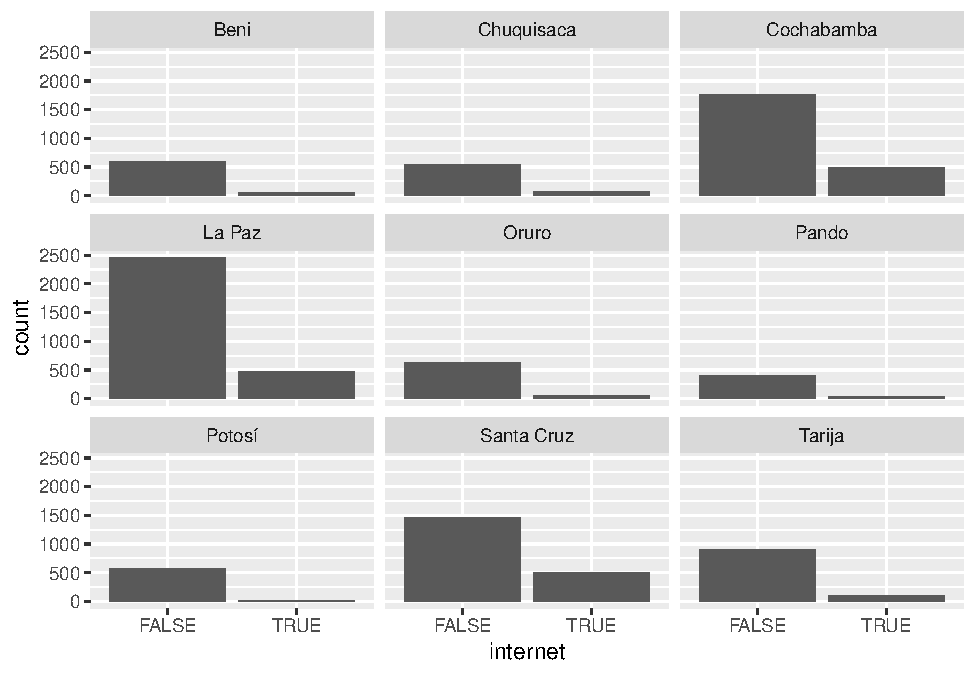
\includegraphics{Parcial_2_sol_files/figure-latex/unnamed-chunk-5-2.pdf}

\end{document}
